\documentclass[a4paper,11pt]{article}
\usepackage{geometry}
 \geometry{
 a4paper,
 total={170mm,257mm},
 left=20mm,
 top=20mm,
 }

 \usepackage{enumerate}
 \usepackage{amsmath}
 \usepackage{siunitx}
 \usepackage{multirow}
\usepackage{colortbl}
 \usepackage{hhline}

 \usepackage{lipsum}  %%% Lorem ipsum
 \usepackage{tikz}

\setlength{\headheight}{30.0pt}
\setlength{\footskip}{20pt}


\usepackage{hyperref}
\hypersetup{
    colorlinks=True,
    linkcolor={blue!20!black},
    filecolor=magenta,      
    urlcolor=cyan,
}



 \usepackage[export]{adjustbox}
\usepackage[english]{babel}
\usepackage[utf8]{inputenc}
\usepackage{fancyhdr}
\usepackage{multicol}

\pagestyle{fancy}
\fancyhf{}
\rhead{\textit{Pul074BEX004}}
\lhead{\textit{Amrit Prasad Phuyal}}
\rfoot{\thepage}


\usepackage{mathpazo} % Palatino font
\usepackage{graphicx}
\usepackage{float}


%%%%%% include  Titles.%%%% use \input{./CP}%%%
%%%use """"""""    \CP{}{}{}{}   """" %%%% and 4 argument to craete Title page 
%%%%%%%%%%%%%%%%%%%%%%%%%%%%%%%%%%%%%%%%%%%%%%%%%%%%%%%%%%%%%%%%%
%%%argument number
%% 1=major header ## Course name 
%% 2=minor4 heading ## lab/assignmet no
%% 3=Title  ## Assignment or Lab title
%% 4=submitted to::## input receiver Name"
%%%%%%%%%%%%%%%%%%%%%%%%%%%%%%%%%%%%%%%%%%%%%%%%%%%%%%%%%%%%%%%%%


\usepackage{mathpazo} % Palatino font
\usepackage{graphicx}
\usepackage{float}

%%% format and command for lab ans c and assembly

\newcommand{\HRule}{\rule{\linewidth}{0.4mm}} % Defines a new command for horizontal lines, change thickness here



%----------------------------------------------------------------------------------------
%	TITLE PAGE
%----------------------------------------------------------------------------------------


\newcommand{\CP}[4]{ \begin{titlepage} % Suppresses displaying the page number on the title page and the subsequent page counts as page 1
		%%%%  univerdity logo%%
		\begin{figure}[H]
			\centering
			
\includegraphics[scale=0.13]{tulogo.jpg}
		\end{figure}
		%%% end university logo

		\center % Centre everything on the page

		%------------------------------------------------
		%	Headings
		%------------------------------------------------

		\textsc{\huge Institute of Engineering \\ Central Campus,Pulchowk}\\[1.5cm] % Main heading such as the name of your university/college

		\textsc{\Large #1}\\[0.5cm] % Major heading such as course name

		\textsc{\large #2}\\[0.5cm] % Minor heading such as assignment no./ lab no.

		%------------------------------------------------
		%	Title
		%------------------------------------------------

		\HRule\\[0.4cm]

		{\Huge\bfseries #3}\\[0.4cm] % Title of your document

		\HRule\\[1.5cm]

		%------------------------------------------------
		%	Author(s)
		%------------------------------------------------
		\vfill\vfill
		\begin{minipage}{0.4\textwidth}
			\begin{flushleft}
				\large{
				\textbf{Submitted BY:}\\
				{\normalsize AMRIT PRASAD PHUYAL}\\ % NAME
				{\normalsize Roll: PULL074BEX004}} % Roll
			\end{flushleft}
		\end{minipage}
		~
		\begin{minipage}{0.4\textwidth}
			\begin{flushright}
				\large
				\textbf{Submitted To:}\\
				{ \normalsize{#4}\\ }% recepent's  Name 
				{\normalsize Department of Electronics and Computer Engineering}
			\end{flushright}
		\end{minipage}

		%------------------------------------------------
		%	Date
		%------------------------------------------------

		\vfill\vfill\vfill % Position the date 3/4 down the remaining page

		{\large\today} % Date, change the \today to a set date if you want to be precise

		\vfill % Push the date up 1/4 of the remaining page

	\end{titlepage}
} %%% cover page

%%% Formating And Command for Embedded Lab  VHDl
%% \ancode{caption}{Filename}


\usepackage{listings}
\usepackage{multicol}
\usepackage{mdframed}

\renewcommand{\lstlistlistingname}{List of MATLAB Codes}
\renewcommand{\lstlistingname}{MATLAB Code}

\setlength{\columnsep}{0.5cm}

\usepackage{xcolor}
\definecolor{codegreen}{rgb}{0,0.6,0}
\definecolor{codegray}{rgb}{0.3,0.3,0.3}
\definecolor{codepurple}{rgb}{0.58,0,0.82}
%\definecolor{backcolour}{rgb}{0.95,0.99,0.92}
\definecolor{backcolour}{rgb}{0,0,0}

\lstdefinestyle{MATLAB}{
  %backgroundcolor=\color{backcolour},  
  commentstyle=\color{codegreen},
  keywordstyle=\color{blue},
  numberstyle=\tiny\color{codegray},
  stringstyle=\color{codepurple},
  basicstyle=\ttfamily\small\color{black},
  breakatwhitespace=false,
  breaklines=true,
  captionpos=b,
  keepspaces=true,
  language=Matlab,
  numbers=left,
  numbersep=5pt,
  showspaces=false,
  frame = single,
  showstringspaces=false,
  showtabs=false,
  tabsize=3
}




\newcommand {\anscode}[2]{
  \lstinputlisting[style=MATLAB,nolol]{#2}

  \begingroup
  \captionof{lstlisting}{#1}
  \endgroup

}

%%% Formating And Command for Embedded Lab  VHDL %%% Matlab code

\newcommand\ddfrac[2]{\frac{\displaystyle #1}{\displaystyle #2}} 



%%%%%%%%%%%%%%%%%%%%%for matlab observation #1 fig name #2 Caption
\newcommand{\mobs}[2]{
    \begin{figure}[H]
        \centering
        \includegraphics[width=1.07\linewidth]{./FIG/#1.eps}
        \caption{#2}
    \end{figure}
   
}

% New command for Figure
\newcommand{\fig}[2]{
    \begin{figure}[H]
        \centering
        \includegraphics[width=0.95\linewidth]{./FIG/#1}
        \caption{#2}
    \end{figure}
}





\begin{document}


%%%%  COver page 
\CP{Digital Signal Processing}{Lab \#6}{Design of FIR Digital Filters using Window method}
{Anila  Kansakar}
%%%%%%%%%%%%%%%%%%%%

\pagenumbering{gobble}
\renewcommand{\contentsname}{Table of Contents}
\tableofcontents

\pagebreak
%\listoffigures
% \pagebreak
% \vspace{5em}
\lstlistoflistings
\vspace{10em}
% \pagebreak
\listoffigures
\pagebreak
\pagenumbering{arabic}

%%%%%%%%%%%%%%%%%%%%%%%%%%%%%%%%%%%%%%%%%%%%%%
\section{Title} {\large Design of FIR Digital Filters using Window method}
%%%%%%%%%%%%%%%%%%%%%%%%%%%%
\section{Objective}
\begin {itemize}
\item To design FIR filter using Window method.
\end{itemize}
%%%%%%%%%%%%%%%%%%%%%


%Theory
\section{Theory}

\section{Background}
In previous experiment we discussed the most commonly used techniques for design of IIR
filters based on transformations of continuous-time IIR systems into discrete time IIR systems.
The major difficulty lies in the implementation of the non-iterative direct design method for IIR
filters. However FIR filters are almost entirely restricted to discrete-time implementations. Thus
the design techniques for FIR filters are based on directly approximating the desired frequency
response of the discrete time system. Furthermore, most techniques for approximating the
magnitude response of the FIR system assume a linear phase constraint; thereby avoiding the
problem of spectrum factorization that complicates the direct design of IIR filters.

The simplest method of FIR design is called the window method. This method generally begins
with an ideal desired frequency response Hd(w). The impulse response hd(n) of the filter
exhibiting this desired frequency response can be obtained from inverse Fourier transform of
Hd(w). However this impulse response exists for n= $-\inf$ to $+\inf$ and hence truncation is needed to
make the finite duration impulse response. The truncation is similar to the multiplication of the
hd(n) with the window function w(n). The multiplication in discrete time domain is equivalent to
the convolution of the two in frequency domain, which actually gives the frequency response of
the truncated FIR filter.

But depending on the tapering of the window to zero at each end, the nature of the window
differs. For example, the rectangular window exhibits the most abrupt changes while
approaching to zero at each end. For the specific value of length of the window, the rectangular
window exhibits main lobe with the greatest width and the lowest side lobe attenuation, than the
other windows like Bartlett, Hanning, Hamming, Blackman etc. There are also adjustable
windows like Kaiser windows whose windowing function w(n) can be adjusted by changing the
value of parameter $\beta$ according to the stop band attenuation A as given below:

\begin{align*}
            & \ 0.1102(A-8.7),                    & if\   A  > 50,           \\
    \beta = & \ 0.5842(A-21)^{0.4}+0.07886(A-21), & if\   21 \leq A \leq 50, \\
            & \ 0.0,                              & if \  A < 21,            \\
            & \text{where}\  A= -20log10 \delta .
\end{align*}

The length of the Kaiser window is given by;
\begin{equation*}
    M = \frac{(\delta-7.95)} {(14.36*\Delta w)} +1, \quad \text{where}\  \frac {\Delta w= (w_s -w_p)}{2}
\end{equation*}




MATLAB Signal Processing Toolbox provides built-in functions to determine and plot the
different types of windowing functions and their frequency responses. For this the functions like
\texttt{Bartlett( ), Hamming( ), Hanning( ), Blackman( ) , Kaiser( )} etc. are available. There is a function
\texttt{fir1( )} that can be used to obtain the frequency response of the designed FIR filter. Use
MATLAB \texttt{‘Help’} for further information of the functions.


\section {Lab Problems}

%%%%%%%%%%%%Problem 111111111111111

\subsection{Problem 1}



\subsection*{Design an FIR linear phase digital filter approximating the ideal frequency response
    \begin{equation*}
        H(w) = \begin{cases}
            1 & |w| \leq \pi/6          \\
            0 & \pi/6 \leq |w| \leq \pi
        \end{cases}
    \end{equation*}
    \begin{enumerate}
        \item Plot the window function for Hamming and its frequency response for length of $M=31$.
        \item Using the Hamming window plot the frequency response of the truncated FIR filter.
        \item Repeat parts (a) and (b) for the Hanning, Blackman and Bartlett windows.
        \item Repeat parts (a), (b) and (d) for filter length of M=61.
    \end{enumerate} }


\MAT{./CODES/p1.m}{Matlab code for FIR linear phase digital filter approximating the ideal frequency response }
\mobs{p11}{Plot window function for Hamming window and its frequency response}
\mobs{p12}{Plot window function for Hanning window and its frequency response}
\mobs{p13}{Plot window function for Blackman window and its frequency response}
\mobs{p14}{Plot window function for Bartlett  window and its frequency response}
\mobs{p15}{Plot window function for Hamming window and its frequency response for length of $M=61$}




%%%%%%%%%%%%Problem 2222222222222222222222

\subsection{Problem 2}



\subsection*{Discuss the effects of different types of the windowing functions on the frequency
    response of the FIR filter. Carry out the comparative study on the basis of the peak side-
    lobe level, the approximate transition width of the main lobe etc. Also discuss on the
    effects of increasing value of M.}


From the observations in the above graphs, the effect of using a different kinds of windowing
functions are seen on the main lobe transition band and the side lobes in the frequency
response of the FIR filter. Here, it can be noted that there is a tradeoff between the width of
the transition band and the attenuation of the side lobes when the windowing function is
varied. In the case of Hamming window, the transition band is slightly increased but has
reduced side lobes in comparison to the Hanning window. The Blackman window has very
small side lobes but has an increased width of the main lobe in comparison to other windows.
Bartlett window has significant side lobes but a lower transition band. The effect of increasing
the size of the window results in an increment of the number of side lobes and a decrement in
the width of the transition band.

%%%%%%%%%%%%Problem 33333333333333333

\subsection{Problem 3}



\subsection*{An analog signal $x(t)$ consists of the sum of two components $x_1(t)$ and $x_2(t)$. The spectral
    characteristics of $x(t)$ is shown in the figure. The signal $x(t)$ is band limited to 40 kHz and is
    sampled at the rate of 100 kHz to yield the sequence $x[n]$.
    \begin{figure*}[h]
        \centering
        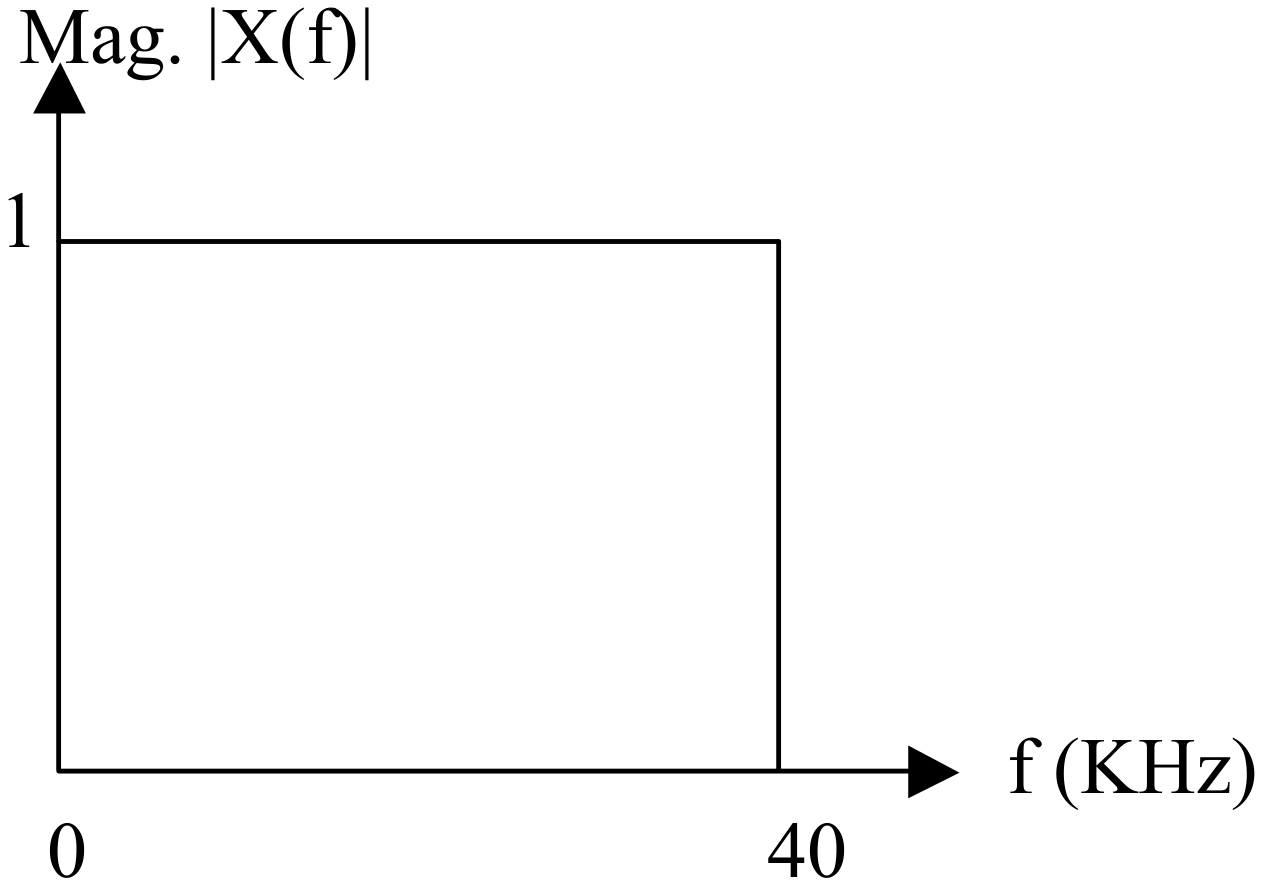
\includegraphics[width=0.5\textwidth]{./FIG/f3.png}
    \end{figure*}
    It is desired to suppress the signal $x_2(t)$ by passing the sequence $x[n]$ through a digital low
    pass filter. The allowable distortion on $|X_1(f)|$ is $\pm 2$\% ($\delta_1=0.02$) over the range $0\leq |f| \leq $ 15 kHz. Above 20 kHz, the filter must have an attenuation of at least 40 DB ($\delta_2=0.01$).
    \begin{enumerate}[a]
        \item For obtaining the filter with above specifications, use the Kaiser window and determine
              the length of the required window. Plot the frequency response of the filter and its
              impulse response also.
        \item If the same filter is to be designed using Hamming window what would be the length of
              the required window. Plot the frequency and impulse response of the filter.
    \end{enumerate}}





\MAT{./CODES/p3.m}{Matlab code for obtaining filter with Kaiser window and its frequency response}
\mobs{p31}{Plot for Frequency Response of the FIR filter using Kaiser window}
\mobs{p32}{Plot for Impulse Response of the FIR filter }




%Discussion and Conclusion
\section{Discussion and Conclusion}
In this lab, we have discussed the different types of windowing functions and their effects on the frequency response of the FIR filter.We explore these properties using various MATLAB functions for the signal processing. We have also discussed the effects of different types of the windowing functions on the frequency response of the FIR filter. We have also discussed the effects of increasing value of M. The effects of using different kinds of windowing functions are seen on the main lobe transition band and the side lobes in the frequency response of the FIR filter. Here, it can be noted that there is a tradeoff between the width of the transition band and the attenuation of the side lobes when the windowing function is varied. Finally we explore Kaiser window and its frequency response.

\end{document}